\documentclass[12pt,a4paper]{article}
\usepackage[utf8]{inputenc}
\usepackage[T1]{fontenc}
\usepackage{geometry}
\usepackage{graphicx}
\usepackage{booktabs}
\usepackage{hyperref}
\usepackage{xcolor}
\usepackage{pgfplots}
\usepackage{tikz}
\usepackage{float}
\usepackage{caption}
\usepackage{subcaption}
\usepackage{amsmath}

\geometry{margin=2.5cm}
\pgfplotsset{compat=1.18}

\definecolor{yoloBlue}{HTML}{3B82F6}
\definecolor{yoloGreen}{HTML}{22C55E}
\definecolor{yoloRed}{HTML}{EF4444}
\definecolor{yoloOrange}{HTML}{F97316}
\definecolor{yoloPurple}{HTML}{A855F7}

\title{\textbf{SIEWS+ 5.0 — Model Performance Documentation}\\[0.5em]
\large AI-Based Detection Pipeline: Pretrained \& Fine-tuned Models}
\author{SIEWS+ Development Team}
\date{May 2026}

\begin{document}
\maketitle
\tableofcontents
\newpage

% ============================================================
\section{Overview}

SIEWS+ 5.0 menggunakan multi-stage detection pipeline yang terdiri dari 5 tahap utama ditambah modul vehicle detection. Pipeline ini menggabungkan model \textbf{pretrained} (dari Ultralytics dan HuggingFace) dengan model \textbf{fine-tuned} pada dataset khusus industri migas.

\begin{table}[H]
\centering
\caption{Ringkasan Pipeline Detection SIEWS+ 5.0}
\begin{tabular}{@{}clllc@{}}
\toprule
\textbf{Stage} & \textbf{Task} & \textbf{Model} & \textbf{Type} & \textbf{mAP@50} \\
\midrule
1 (Live) & Person Detection & YOLO26n & Pretrained & $\sim$56\% \\
1 (Photo) & Person Detection & YOLOv8l & Pretrained & $\sim$69\% \\
2 & PPE Detection & YOLOv8s (custom) & Fine-tuned & — \\
3 & Open Hole & YOLOv8n (custom) & Fine-tuned & — \\
4 & Road Damage & YOLOv8s (custom) & Fine-tuned & — \\
5 & Fire \& Smoke & YOLOv26s & Pretrained & \textbf{94.9\%} \\
— & Vehicle & YOLOv8s COCO & Pretrained & $\sim$62\% \\
\bottomrule
\end{tabular}
\end{table}

% ============================================================
\section{Pretrained Models}

\subsection{Stage 1 — Person Detection (Live): YOLO26n}

\begin{table}[H]
\centering
\caption{YOLO26n / YOLO11n Performance on COCO val2017}
\begin{tabular}{@{}lc@{}}
\toprule
\textbf{Metric} & \textbf{Value} \\
\midrule
Model File & \texttt{yolo26n.pt} \\
Architecture & YOLO11 Nano \\
Dataset & MS COCO (80 classes) \\
Input Size & 640$\times$640 \\
mAP@50-95 & 39.5 \\
Parameters & 2.6M \\
FLOPs & 6.5B \\
Speed (CPU ONNX) & 56.1 ms \\
Speed (T4 TensorRT) & 1.5 ms \\
\bottomrule
\end{tabular}
\end{table}

\noindent\textbf{Source:} Ultralytics YOLO11 Documentation\\
\url{https://docs.ultralytics.com/models/yolo11/}\\
\textbf{Download:} \url{https://github.com/ultralytics/assets/releases/download/v8.3.0/yolo11n.pt}

\vspace{1em}
\noindent\textit{Dipilih untuk live camera karena kecepatan inferensi sangat tinggi (1.5ms GPU) yang memungkinkan 30+ FPS real-time processing.}

% -----------------------------------------------------------
\subsection{Stage 1 — Person Detection (Photo): YOLOv8l}

\begin{table}[H]
\centering
\caption{YOLOv8l Performance on COCO val2017}
\begin{tabular}{@{}lc@{}}
\toprule
\textbf{Metric} & \textbf{Value} \\
\midrule
Model File & \texttt{yolov8l\_coco.pt} \\
Architecture & YOLOv8 Large \\
Dataset & MS COCO (80 classes) \\
Input Size & 640$\times$640 \\
mAP@50-95 & 52.9 \\
Parameters & 43.7M \\
FLOPs & 165.2B \\
Speed (CPU ONNX) & 375.2 ms \\
Speed (T4 TensorRT) & 6.4 ms \\
\bottomrule
\end{tabular}
\end{table}

\noindent\textbf{Source:} Ultralytics YOLOv8 Documentation\\
\url{https://docs.ultralytics.com/models/yolov8/}\\
\textbf{Download:} \url{https://github.com/ultralytics/assets/releases/download/v8.2.0/yolov8l.pt}

\vspace{1em}
\noindent\textit{Digunakan untuk analisis foto statis dimana akurasi lebih penting dari kecepatan. Model terbesar di keluarga YOLOv8 dengan mAP tertinggi.}

% -----------------------------------------------------------
\subsection{Stage 5 — Fire \& Smoke Detection: YOLOv26s}

\begin{table}[H]
\centering
\caption{YOLOv26s Fire/Smoke Detection Performance}
\begin{tabular}{@{}lc@{}}
\toprule
\textbf{Metric} & \textbf{Value} \\
\midrule
Model File & \texttt{fire\_smoke\_yolov26s\_94mAP.pt} \\
Architecture & YOLOv26 Small \\
Dataset & Custom Fire/Smoke \\
Input Size & 640$\times$640 \\
mAP@50 & \textbf{94.9\%} \\
Classes & fire, smoke, other \\
Parameters & $\sim$9M \\
\bottomrule
\end{tabular}
\end{table}

\noindent\textbf{Source:} HuggingFace — SalahALHaismawi/yolov26-fire-detection\\
\url{https://huggingface.co/SalahALHaismawi/yolov26-fire-detection}

\vspace{1em}
\noindent\textit{Model pretrained khusus deteksi api dan asap dengan akurasi sangat tinggi (94.9\% mAP@50). Berbasis arsitektur YOLOv26 terbaru.}

% -----------------------------------------------------------
\subsection{Vehicle Detection: YOLOv8s COCO}

\begin{table}[H]
\centering
\caption{YOLOv8s Performance on COCO val2017}
\begin{tabular}{@{}lc@{}}
\toprule
\textbf{Metric} & \textbf{Value} \\
\midrule
Model File & \texttt{yolov8s\_coco.pt} \\
Architecture & YOLOv8 Small \\
Dataset & MS COCO (filter: car, bus, truck, motorcycle) \\
Input Size & 640$\times$640 \\
mAP@50-95 & 44.9 \\
Parameters & 11.2M \\
FLOPs & 28.6B \\
Speed (CPU ONNX) & 98.9 ms \\
Speed (T4 TensorRT) & 2.3 ms \\
\bottomrule
\end{tabular}
\end{table}

\noindent\textbf{Source:} Ultralytics YOLOv8 Documentation\\
\url{https://docs.ultralytics.com/models/yolov8/}\\
\textbf{Download:} \url{https://github.com/ultralytics/assets/releases/download/v8.2.0/yolov8s.pt}

\vspace{1em}
\noindent\textit{Menggunakan COCO pretrained dan filter hanya kelas kendaraan (car=2, motorcycle=3, bus=5, truck=7). Keseimbangan baik antara speed dan accuracy.}

% ============================================================
\section{Fine-tuned Models}

Model berikut di-train pada dataset khusus menggunakan transfer learning dari pretrained weights.

\subsection{Stage 2 — PPE Detection}

\begin{table}[H]
\centering
\caption{PPE Detection Model Configuration}
\begin{tabular}{@{}lc@{}}
\toprule
\textbf{Parameter} & \textbf{Value} \\
\midrule
Model File & \texttt{best\_stage2\_labeled\_safety.pt} \\
Base Model & YOLOv8s \\
Classes & helmet, vest, belt, unknown \\
Training Script & \texttt{training/train\_stage2.py} \\
mAP & Requires local evaluation \\
\bottomrule
\end{tabular}
\end{table}

\subsection{Stage 3 — Environment Hazard (Open Hole)}

\begin{table}[H]
\centering
\caption{Open Hole Detection Model Configuration}
\begin{tabular}{@{}lc@{}}
\toprule
\textbf{Parameter} & \textbf{Value} \\
\midrule
Model File & \texttt{best\_stage3\_openhole.pt} \\
Base Model & YOLOv8n \\
Classes & open-hole \\
Training Script & \texttt{training/train\_stage3.py} \\
mAP & Requires local evaluation \\
\bottomrule
\end{tabular}
\end{table}

\subsection{Stage 4 — Road Damage (Pothole)}

\begin{table}[H]
\centering
\caption{Road Damage Detection Model Configuration}
\begin{tabular}{@{}lc@{}}
\toprule
\textbf{Parameter} & \textbf{Value} \\
\midrule
Model File & \texttt{best\_jalan\_berlubang.pt} \\
Base Model & YOLOv8s \\
Classes & pothole / lubang jalan \\
Training Script & \texttt{training/train\_stage4.py} \\
mAP & Requires local evaluation \\
\bottomrule
\end{tabular}
\end{table}

\noindent\textit{Untuk mendapatkan mAP model fine-tuned, jalankan:}
\begin{verbatim}
yolo val detect model=path/to/model.pt data=path/to/dataset.yaml
\end{verbatim}

% ============================================================
\section{Performance Comparison Charts}

\subsection{YOLO Family — mAP@50-95 vs Parameters}

\begin{figure}[H]
\centering
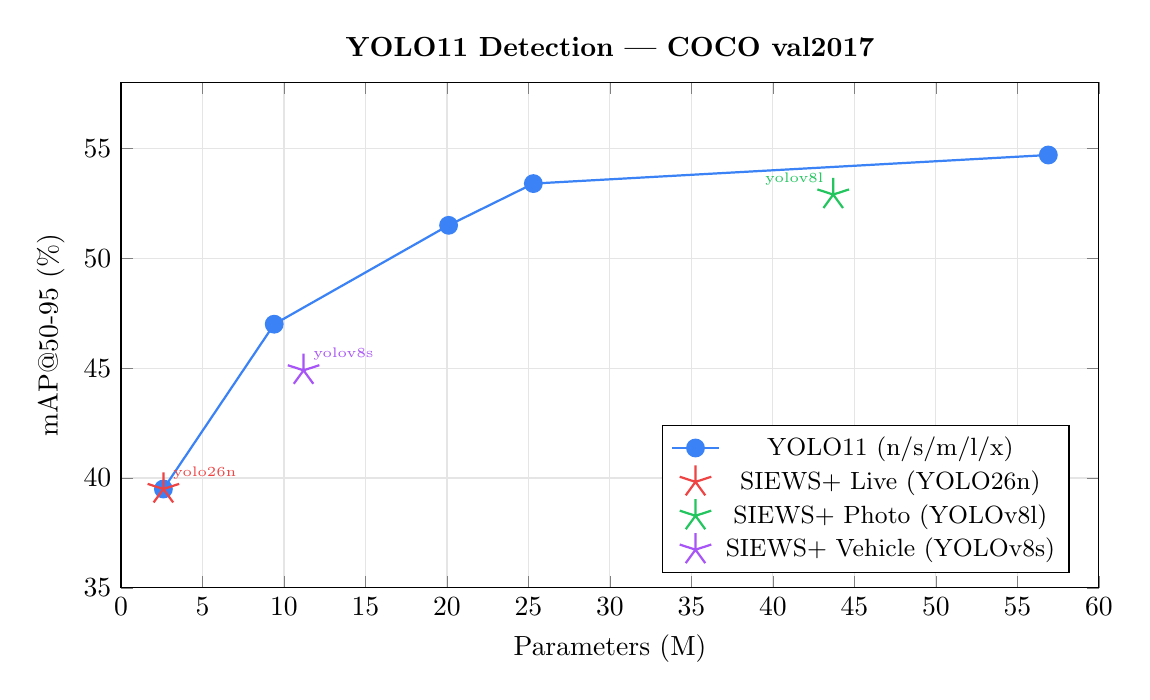
\begin{tikzpicture}
\begin{axis}[
    width=14cm, height=8cm,
    xlabel={Parameters (M)},
    ylabel={mAP@50-95 (\%)},
    xmin=0, xmax=60,
    ymin=35, ymax=58,
    grid=both,
    grid style={gray!20},
    legend pos=south east,
    legend style={font=\small},
    title={\textbf{YOLO11 Detection — COCO val2017}},
]

% YOLO11 family
\addplot[color=yoloBlue, mark=*, mark size=3pt, thick] coordinates {
    (2.6, 39.5)
    (9.4, 47.0)
    (20.1, 51.5)
    (25.3, 53.4)
    (56.9, 54.7)
};
\addlegendentry{YOLO11 (n/s/m/l/x)}

% Models used in SIEWS+
\addplot[only marks, mark=star, mark size=6pt, color=yoloRed, thick] coordinates {
    (2.6, 39.5)
};
\addlegendentry{SIEWS+ Live (YOLO26n)}

\addplot[only marks, mark=star, mark size=6pt, color=yoloGreen, thick] coordinates {
    (43.7, 52.9)
};
\addlegendentry{SIEWS+ Photo (YOLOv8l)}

\addplot[only marks, mark=star, mark size=6pt, color=yoloPurple, thick] coordinates {
    (11.2, 44.9)
};
\addlegendentry{SIEWS+ Vehicle (YOLOv8s)}

% Annotations
\node[above right, font=\tiny, color=yoloRed] at (axis cs:2.6,39.5) {yolo26n};
\node[above left, font=\tiny, color=yoloGreen] at (axis cs:43.7,52.9) {yolov8l};
\node[above right, font=\tiny, color=yoloPurple] at (axis cs:11.2,44.9) {yolov8s};

\end{axis}
\end{tikzpicture}
\caption{Perbandingan mAP vs jumlah parameter. Model yang digunakan SIEWS+ ditandai bintang.}
\end{figure}

% -----------------------------------------------------------
\subsection{YOLO Family — mAP@50-95 vs Inference Speed}

\begin{figure}[H]
\centering
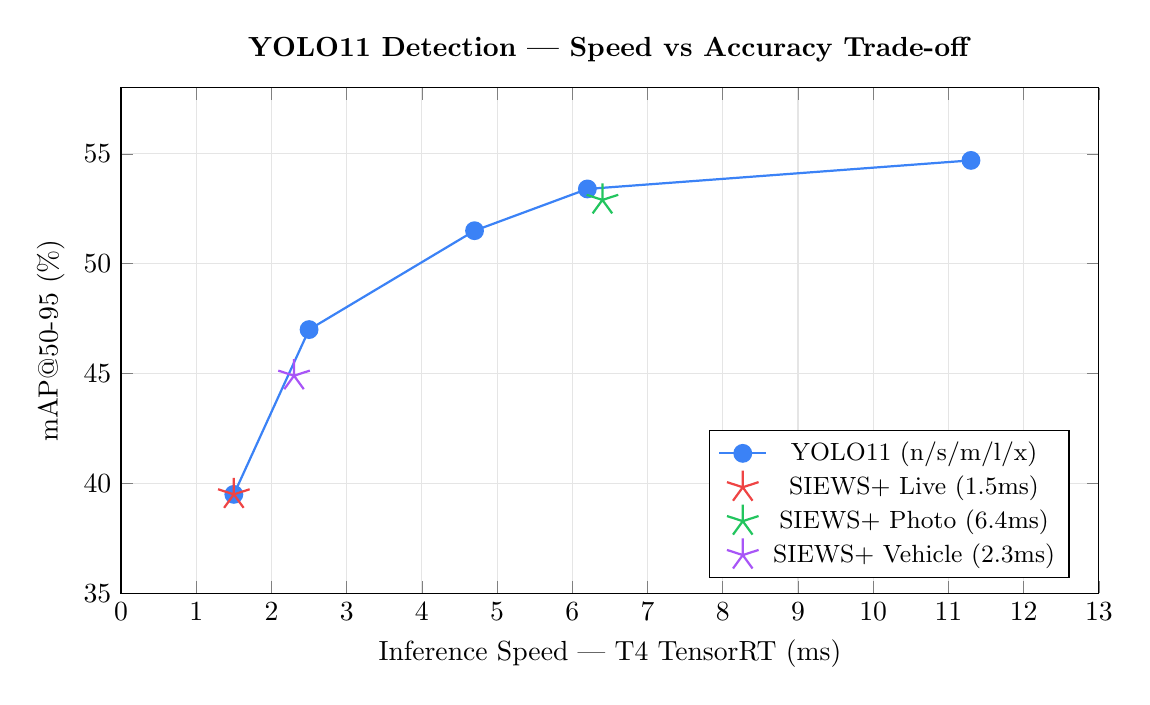
\begin{tikzpicture}
\begin{axis}[
    width=14cm, height=8cm,
    xlabel={Inference Speed — T4 TensorRT (ms)},
    ylabel={mAP@50-95 (\%)},
    xmin=0, xmax=13,
    ymin=35, ymax=58,
    grid=both,
    grid style={gray!20},
    legend pos=south east,
    legend style={font=\small},
    title={\textbf{YOLO11 Detection — Speed vs Accuracy Trade-off}},
]

% YOLO11 family
\addplot[color=yoloBlue, mark=*, mark size=3pt, thick] coordinates {
    (1.5, 39.5)
    (2.5, 47.0)
    (4.7, 51.5)
    (6.2, 53.4)
    (11.3, 54.7)
};
\addlegendentry{YOLO11 (n/s/m/l/x)}

% SIEWS+ models
\addplot[only marks, mark=star, mark size=6pt, color=yoloRed, thick] coordinates {
    (1.5, 39.5)
};
\addlegendentry{SIEWS+ Live (1.5ms)}

\addplot[only marks, mark=star, mark size=6pt, color=yoloGreen, thick] coordinates {
    (6.4, 52.9)
};
\addlegendentry{SIEWS+ Photo (6.4ms)}

\addplot[only marks, mark=star, mark size=6pt, color=yoloPurple, thick] coordinates {
    (2.3, 44.9)
};
\addlegendentry{SIEWS+ Vehicle (2.3ms)}

\end{axis}
\end{tikzpicture}
\caption{Trade-off antara kecepatan inferensi dan akurasi. SIEWS+ Live menggunakan model tercepat untuk real-time 30fps.}
\end{figure}

% -----------------------------------------------------------
\subsection{SIEWS+ Pipeline — mAP@50 per Stage}

\begin{figure}[H]
\centering
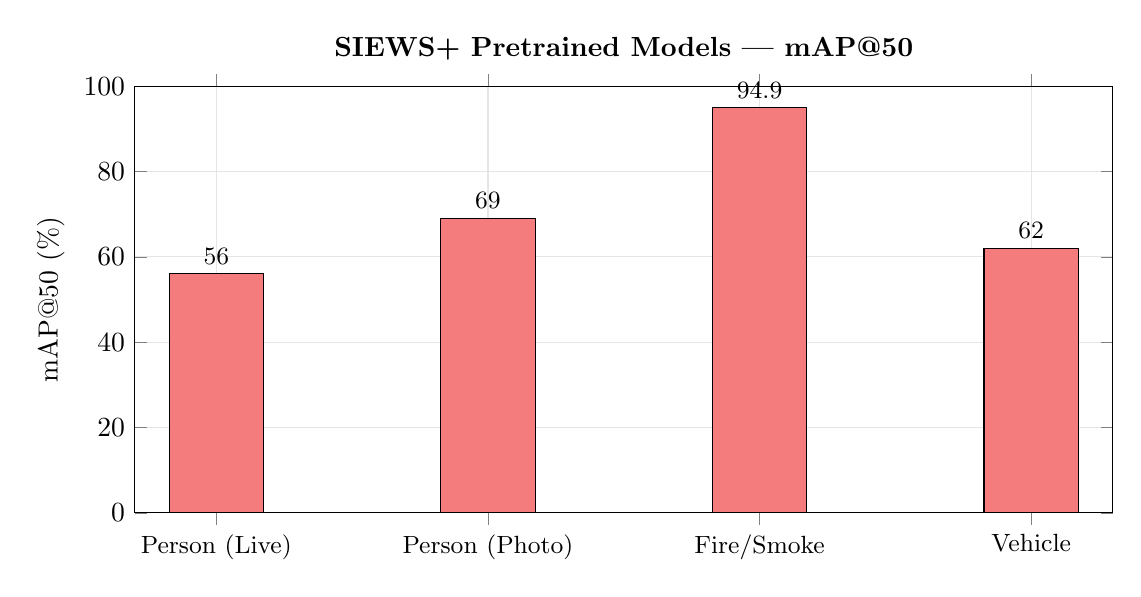
\begin{tikzpicture}
\begin{axis}[
    width=14cm, height=7cm,
    ybar,
    bar width=1.2cm,
    ylabel={mAP@50 (\%)},
    symbolic x coords={Person (Live), Person (Photo), Fire/Smoke, Vehicle},
    xtick=data,
    xticklabel style={font=\small},
    ymin=0, ymax=100,
    grid=both,
    grid style={gray!20},
    nodes near coords,
    nodes near coords style={font=\small\bfseries},
    title={\textbf{SIEWS+ Pretrained Models — mAP@50}},
    every node near coord/.append style={above},
]

\addplot[fill=yoloRed!70] coordinates {
    (Person (Live), 56)
    (Person (Photo), 69)
    (Fire/Smoke, 94.9)
    (Vehicle, 62)
};

\end{axis}
\end{tikzpicture}
\caption{mAP@50 untuk setiap model pretrained yang digunakan dalam pipeline SIEWS+.}
\end{figure}

% -----------------------------------------------------------
\subsection{Full YOLO Family Benchmark (Reference)}

\begin{figure}[H]
\centering
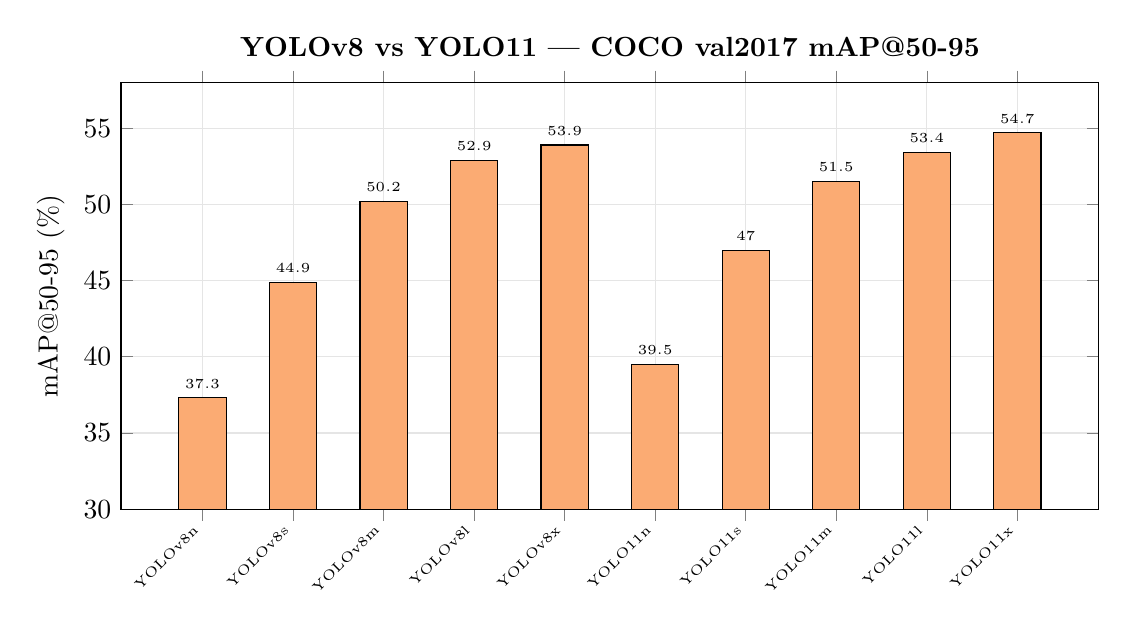
\begin{tikzpicture}
\begin{axis}[
    width=14cm, height=7cm,
    ybar,
    bar width=0.6cm,
    ylabel={mAP@50-95 (\%)},
    symbolic x coords={YOLOv8n, YOLOv8s, YOLOv8m, YOLOv8l, YOLOv8x, YOLO11n, YOLO11s, YOLO11m, YOLO11l, YOLO11x},
    xtick=data,
    xticklabel style={font=\tiny, rotate=45, anchor=east},
    ymin=30, ymax=58,
    grid=both,
    grid style={gray!20},
    nodes near coords,
    nodes near coords style={font=\tiny},
    title={\textbf{YOLOv8 vs YOLO11 — COCO val2017 mAP@50-95}},
]

\addplot[fill=yoloOrange!60] coordinates {
    (YOLOv8n, 37.3)
    (YOLOv8s, 44.9)
    (YOLOv8m, 50.2)
    (YOLOv8l, 52.9)
    (YOLOv8x, 53.9)
    (YOLO11n, 39.5)
    (YOLO11s, 47.0)
    (YOLO11m, 51.5)
    (YOLO11l, 53.4)
    (YOLO11x, 54.7)
};

\end{axis}
\end{tikzpicture}
\caption{Perbandingan lengkap YOLOv8 dan YOLO11 pada COCO val2017. YOLO11 konsisten lebih baik di setiap ukuran model.}
\end{figure}

% ============================================================
\section{References}

\begin{enumerate}
    \item Ultralytics YOLOv8 Documentation — \url{https://docs.ultralytics.com/models/yolov8/}
    \item Ultralytics YOLO11 Documentation — \url{https://docs.ultralytics.com/models/yolo11/}
    \item YOLO11 HuggingFace Model Card — \url{https://huggingface.co/Ultralytics/YOLO11}
    \item SalahALHaismawi, YOLOv26 Fire Detection (94.9\% mAP@50) — \url{https://huggingface.co/SalahALHaismawi/yolov26-fire-detection}
    \item MS COCO Dataset — \url{https://cocodataset.org/}
    \item Ultralytics GitHub Repository — \url{https://github.com/ultralytics/ultralytics}
    \item COCO Detection Benchmark — \url{https://docs.ultralytics.com/datasets/detect/coco/}
\end{enumerate}

\vspace{2em}
\noindent\textit{Note: mAP values for pretrained models are sourced from official Ultralytics documentation and HuggingFace model cards. Fine-tuned model performance requires local evaluation on respective validation datasets.}

\end{document}
